\documentclass{article}

%%%%
% PLOTS mapas y conglomerados
%%%%


\usepackage[utf8]{inputenc}
\usepackage{longtable}
\usepackage{authblk}
\usepackage{adjustbox}
\usepackage{natbib}


\title{LOS INDICES DEL MUNDO}
% autores
\renewcommand\Authand{, y }
\author[1]{\normalsize Estrella DelCurso}
\author[2]{\normalsize Prossimo Deal Lado}

\affil[1,2]{\small  Escuela de Ingenieri<U+0301>a,Universidad de los Andes\\
\texttt{{delcurso,deallado}@uniandes.edu.col}}
\affil[1]{\small Instituto de altas investigaciones financieras\\
Banco del Parque\\
\texttt{delcurso@bp.com.col}}

\date{30 de Junio de 2018}

%%%%
\usepackage{Sweave}
\begin{document}
\Sconcordance{concordance:paperVersion_7_matriz.tex:paperVersion_7_matriz.Rnw:%
1 29 1 1 0 29 1}


\maketitle


\begin{abstract}
Este es mi primer trabajo en exploracion y modelamiento de indices usando LATEX. Este trabajo lo he hecho bajo la filosofi<U+0301>a de trabajo replicable. Este es mi primer trabajo en exploracion y modelamiento de indices usando LATEX. Este trabajo lo he hecho bajo la filosofi<U+0301>a de trabajo replicable. Este es mi primer trabajo en exploracion y modelamiento de indices usando LATEX. Este trabajo lo he hecho bajo la filosofi<U+0301>a de trabajo replicable. Este es mi primer trabajo en exploracion y modelamiento de indices usando LATEX. Este trabajo lo he hecho bajo la filosofi<U+0301>a de trabajo replicable.
\end{abstract}

\section*{Introduccio<U+0301>n}

Aqui les presento mi investigacion sobre diversos indices sociales en el mundo. Los indices los consegui<U+0301> de wikipedia, espero que les gusten mucho. Aqui les presento mi investigacion sobre diversos indices sociales en el mundo. Los indices los consegui<U+0301> de wikipedia, espero que les gusten mucho.Aqui les presento mi investigacion sobre diversos indices sociales en el mundo. Los indices los consegui<U+0301> de wikipedia, espero que les gusten mucho.Aqui les presento mi investigacion sobre diversos indices sociales en el mundo. Los indices los consegui<U+0301> de wikipedia, espero que les gusten mucho.
Aqui les presento mi investigacion sobre diversos indices sociales en el mundo. Los indices los consegui<U+0301> de wikipedia, espero que les gusten mucho.Aqui les presento mi investigacion sobre diversos indices sociales en el mundo. Los indices los consegui<U+0301> de wikipedia, espero que les gusten mucho.Aqui les presento mi investigacion sobre diversos indices sociales en el mundo. Los indices los consegui<U+0301> de wikipedia, espero que les gusten mucho.

Comencemos viendo que hay en la seccio<U+0301>n \ref{univariada} en la pa<U+0301>gina \pageref{univariada}.

\clearpage


NA

NA



\begin{Schunk}
\begin{Soutput}
[1] NA
\end{Soutput}
\end{Schunk}


NA

% latex table generated in R 3.5.0 by xtable 1.8-2 package
% Fri Jun 29 15:59:52 2018
\begingroup\normalsize
\begin{longtable}{llrrr}
\caption{Tablas de Frecuencia de la variables en estudio} \\ 
 \textbf{Variable} & \textbf{Levels} & $\mathbf{n}$ & $\mathbf{\%}$ & $\mathbf{\sum \%}$ \\ 
  \hline \hline
WorldFreedom & 1 & 55 & 26.7 & 26.7 \\ 
   & 3 & 62 & 30.1 & 56.8 \\ 
   & 5 & 89 & 43.2 & 100.0 \\ 
   \hline
 & all & 206 & 100.0 &  \\ 
   \hline
\hline
EconomicFreedom & 1 & 21 & 10.1 & 10.1 \\ 
   & 2 & 78 & 37.7 & 47.8 \\ 
   & 3 & 74 & 35.8 & 83.6 \\ 
   & 4 & 28 & 13.5 & 97.1 \\ 
   & 5 & 6 & 2.9 & 100.0 \\ 
   \hline
 & all & 207 & 100.0 &  \\ 
   \hline
\hline
PressFreedom & 1 & 22 & 10.7 & 10.7 \\ 
   & 2 & 53 & 25.7 & 36.4 \\ 
   & 3 & 66 & 32.0 & 68.5 \\ 
   & 4 & 48 & 23.3 & 91.8 \\ 
   & 5 & 17 & 8.2 & 100.0 \\ 
   \hline
 & all & 206 & 100.0 &  \\ 
   \hline
\hline
Democracy & 1 & 60 & 29.1 & 29.1 \\ 
   & 2 & 45 & 21.8 & 51.0 \\ 
   & 4 & 82 & 39.8 & 90.8 \\ 
   & 5 & 19 & 9.2 & 100.0 \\ 
   \hline
 & all & 206 & 100.0 &  \\ 
   \hline
\hline
\hline
\label{Tfrecuencias}
\end{longtable}
\endgroup

NA

\clearpage

NA


%%%%% figure
\begin{figure}[h]
\centering
\begin{Schunk}
\begin{Soutput}
[1] NA
\end{Soutput}
\end{Schunk}
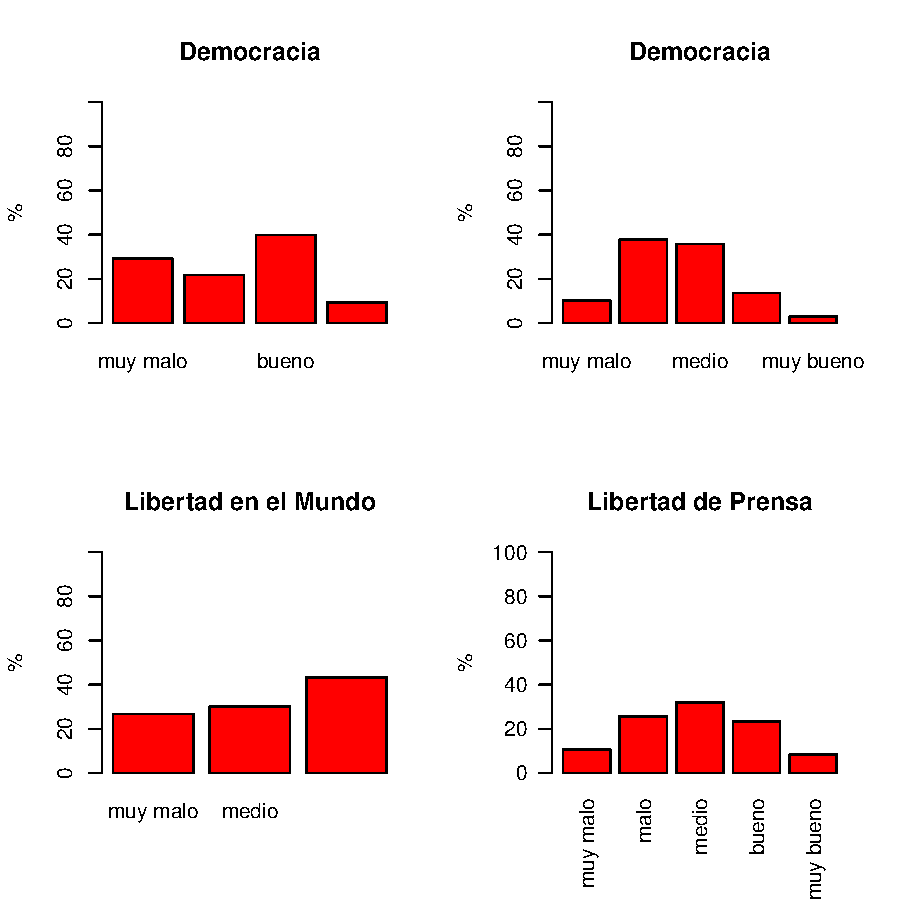
\includegraphics{paperVersion_7_univariada-barplots}
NA
\label{barplots}
\end{figure}

NA

[1] NA




\endinput

NA

NA

\begin{Schunk}
\begin{Soutput}
[1] NA
\end{Soutput}
\end{Schunk}

[1] NA

NA


[1] NA
Lo visto en la Tabla \ref{corrTableX} se refuerza claramente en la Figura \ref{corrPlotX}.

\begin{figure}[h]
\centering
\begin{adjustbox}{width=7cm,height=7cm,clip,trim=1.5cm 0.5cm 0cm 1.5cm}
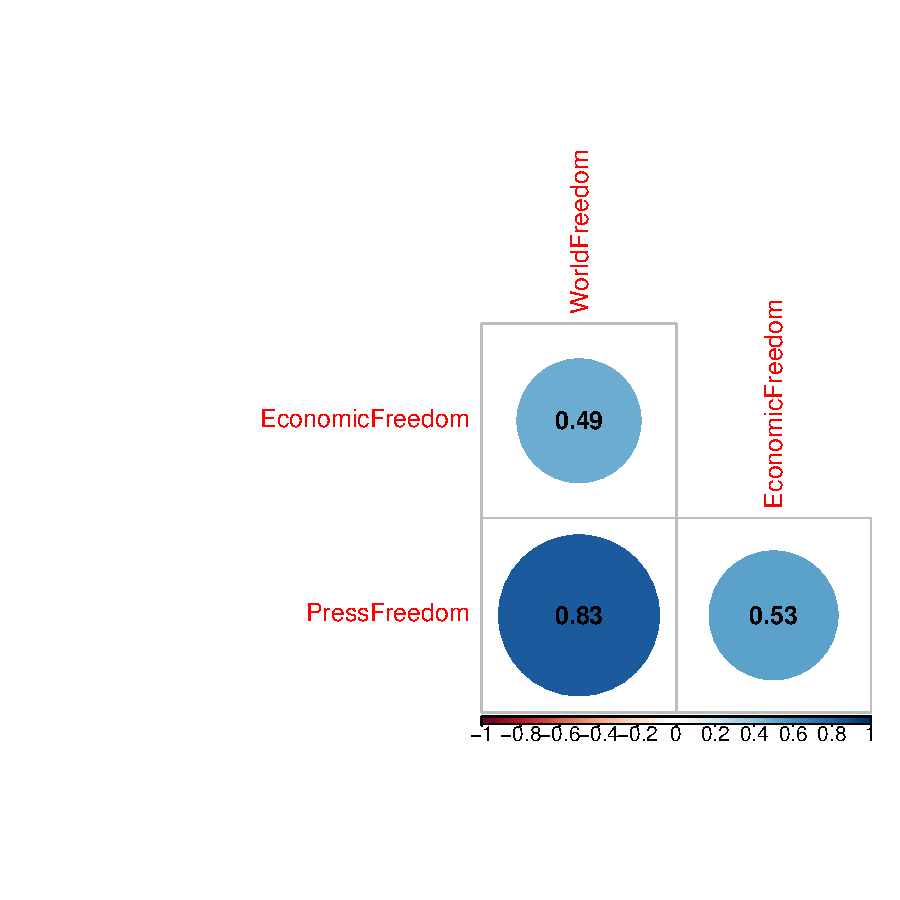
\includegraphics{paperVersion_7_bivariada-corrPlotX}
\end{adjustbox}
NA
\label{corrPlotX}
\end{figure}



\endinput

\section{Modelos de Regresi<U+00F3>n}

Finalmente, vemos los modelos propuestos. Primero sin la libertad mundial como independiente, y luego con est<U+00E1>. Los resultados se muestran en la Tabla \ref{regresiones} de la p<U+00E1>gina \pageref{regresiones}.




% Table created by stargazer v.5.2.2 by Marek Hlavac, Harvard University. E-mail: hlavac at fas.harvard.edu
% Date and time: Fri, Jun 29, 2018 - 16:02:46
\begin{table}[!htbp] \centering 
  \caption{Modelos de Regresi<U+00F3>n} 
  \label{regresiones} 
\begin{tabular}{@{\extracolsep{5pt}}lcc} 
\\[-1.8ex]\hline 
\hline \\[-1.8ex] 
 & \multicolumn{2}{c}{\textit{Dependent variable:}} \\ 
\cline{2-3} 
\\[-1.8ex] & \multicolumn{2}{c}{Democracy} \\ 
\\[-1.8ex] & (1) & (2)\\ 
\hline \\[-1.8ex] 
 WorldFreedom &  & 0.704$^{***}$ \\ 
  &  & (0.046) \\ 
  & & \\ 
 EconomicFreedom & 0.377$^{***}$ & 0.291$^{***}$ \\ 
  & (0.077) & (0.053) \\ 
  & & \\ 
 PressFreedom & 0.833$^{***}$ & 0.012 \\ 
  & (0.065) & (0.070) \\ 
  & & \\ 
 Constant & $-$0.642$^{***}$ & $-$0.354$^{**}$ \\ 
  & (0.199) & (0.138) \\ 
  & & \\ 
\hline \\[-1.8ex] 
Observations & 206 & 206 \\ 
R$^{2}$ & 0.637 & 0.830 \\ 
Adjusted R$^{2}$ & 0.634 & 0.828 \\ 
Residual Std. Error & 0.880 (df = 203) & 0.603 (df = 202) \\ 
F Statistic & 178.197$^{***}$ (df = 2; 203) & 329.420$^{***}$ (df = 3; 202) \\ 
\hline 
\hline \\[-1.8ex] 
\textit{Note:}  & \multicolumn{2}{r}{$^{*}$p$<$0.1; $^{**}$p$<$0.05; $^{***}$p$<$0.01} \\ 
\end{tabular} 
\end{table} 
Como se vi<U+00F3> en la Tabla \ref{regresiones}, cuando est<U+00E1> presente el \emph{indice de libertad mundial}, el \emph{<U+00ED>ndice de libertad de prensa} pierde significancia.

\clearpage

\section{Exploraci<U+00F3>n Espacial}

Como acabamos de ver en la Tabla \ref{regresiones} en la p<U+00E1>gina \pageref{regresiones}, si quisieras sintetizar la multidimensionalidad de nuestros indicadores, podr<U+00ED>amos usar tres de las cuatro variables que tenemos (un par de las originales tiene demasiada correlaci<U+00F3>n). 

As<U+00ED>, propongo que calculemos conglomerados de pa<U+00ED>ses usando toda la informaci<U+00F3>n de tres de los indicadores. Como nuestras variables son ordinales utilizaremos un proceso de conglomeraci<U+00F3>n donde las distancia ser<U+00E1>n calculadas usando la medida {\bf gower} propuestas en \cite{gower_general_1971}, y para los enlazamientos usaremos la t<U+00E9>cnica de {\bf medoides} seg<U+00FA>n \cite{reynolds_clustering_2006}. Los tres conglomerados se muestran en la Figura \ref{clustmap}.






\begin{figure}[h]
\centering
\begin{adjustbox}{width=11cm,height=8cm,clip,trim=1cm 2.5cm 0cm 2.5cm}
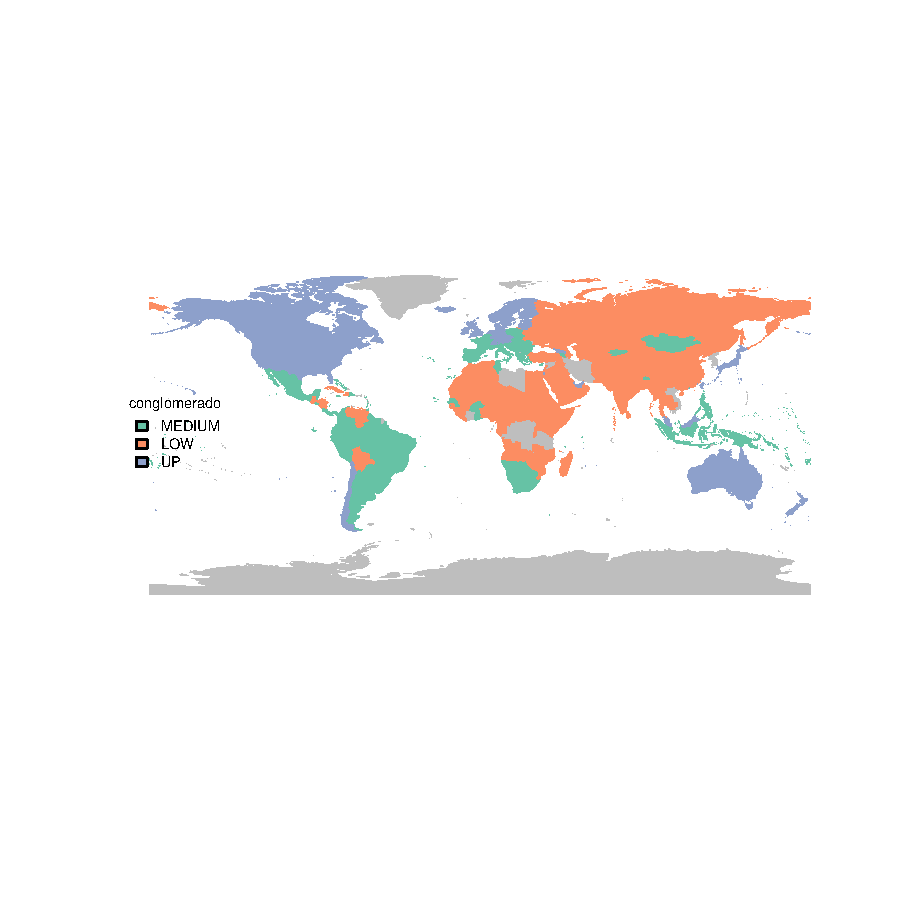
\includegraphics{paperVersion_7_regresion-plotMap1}
\end{adjustbox}
\caption{Paises conglomerados segun sus indicadores sociopol<U+00ED>ticos}\label{clustmap}
\end{figure}



\endinput



\bibliographystyle{apalike}
\renewcommand{\refname}{Bibliography}
\bibliography{Colombia}

\end{document}
